\documentclass[12pt]{article}

\usepackage[utf8]{inputenc}
\usepackage{latexsym,amsfonts,amssymb,amsthm,amsmath}

\setlength{\parindent}{0in}
\setlength{\oddsidemargin}{0in}
\setlength{\textwidth}{6.5in}
\setlength{\textheight}{8.8in}
\setlength{\topmargin}{0in}
\setlength{\headheight}{18pt}
\usepackage{graphicx} % Required for inserting images
\usepackage{enumitem}
\usepackage{listings}

\usepackage{xcolor}

\usepackage{booktabs}

\usepackage{tikz}
\usepackage{pgfplots}
\pgfplotsset{compat=1.18}

\usepackage[toc]{appendix}

\title{Econometría 2502 - Taller 2}
\author{Rafael Marulanda, Carlos Puerto y Lorena Toro}
\date{27 de setiembre de 2025}

\begin{document}

\maketitle

\section{Ejercicio sobre la base de datos \texttt{wage1}}

Descargue la base de datos \texttt{wage1}.

\begin{enumerate}[label=\alph*)]
    \item Calcule estadísticas descriptivas de \texttt{wage}, \texttt{educ}, \texttt{exper}, \texttt{tenure} y \texttt{numdep}. Muestre sus resultados. Calcule el histograma de frecuencias de cada una de las variables. Interprete sus resultados.
    
    \item Tabule y calcule las estadísticas descriptivas de las variables \texttt{nonwhite}, \texttt{female} y \texttt{married}. Interprete sus resultados.
    
    \item Calcule el número de mujeres no blancas en la muestra.
    
    \item Calcule el número de hombres blancos y casados de la muestra.
    
    \item Calcule el número de mujeres blancas y solteras en la muestra.
    
    \item Calcule la covarianza y la correlación entre \texttt{wage}, \texttt{educ}, \texttt{exper}, \texttt{tenure} y \texttt{numdep}.
\end{enumerate}

\section{Análisis de Estadísticas Descriptivas y Distribuciones de Frecuencia}

\subsection{Resumen de las Distribuciones de Variables}

Este apartado presenta un análisis exhaustivo de las estadísticas descriptivas y distribuciones de frecuencia para las variables principales del conjunto de datos wage1. La Tabla \ref{tab:descriptive_statistics} proporciona las estadísticas resumen para las variables continuas bajo examen: salarios por hora, años de educación, experiencia en el mercado laboral, antigüedad en el empleo y número de dependientes económicos.

%\begin{table}[htbp]\centering
\def\sym#1{\ifmmode^{#1}\else\(^{#1}\)\fi}
\caption{Descriptive Statistics}
\begin{tabular}{l*{1}{ccccc}}
\toprule
                    &\multicolumn{5}{c}{(1)}                                         \\
                    &\multicolumn{5}{c}{}                                            \\
                    &        mean&          sd&         min&         max&       count\\
\midrule
average hourly earnings&        5.90&        3.69&        0.53&       24.98&      526.00\\
years of education  &       12.56&        2.77&        0.00&       18.00&      526.00\\
years potential experience&       17.02&       13.57&        1.00&       51.00&      526.00\\
years with current employer&        5.10&        7.22&        0.00&       44.00&      526.00\\
number of dependents&        1.04&        1.26&        0.00&        6.00&      526.00\\
\midrule
Observations        &         526&            &            &            &            \\
\bottomrule
\end{tabular}
\end{table}


\subsection{Análisis de la Distribución Salarial}

La variable de salario, medida en dólares por hora, presenta una media de \$5.90 con una desviación estándar de \$3.69, como se muestra en la Tabla \ref{tab:descriptive_statistics}. La distribución demuestra un sesgo positivo pronunciado, evidenciado por la diferencia sustancial entre la media (\$5.90) y la mediana (\$4.65). Este sesgo hacia la derecha indica que mientras la mayoría de los trabajadores perciben salarios modestos, una pequeña proporción de trabajadores con altos ingresos influye significativamente en el promedio hacia arriba. El rango intercuartílico abarca desde \$3.33 hasta \$6.88, sugiriendo que el cincuenta por ciento de la fuerza laboral gana dentro de esta banda relativamente estrecha.

La Figura \ref{fig:hist_wage} ilustra la distribución de frecuencias de los salarios, revelando una concentración de observaciones en el rango de \$2-\$6 con una cola larga hacia la derecha que se extiende hasta el valor máximo de \$24.98. El coeficiente de variación, calculado en 62.5\%, indica una variabilidad relativa sustancial en los salarios a través de la muestra. Este patrón se alinea con los fenómenos de desigualdad salarial bien documentados en la literatura de economía laboral, donde las diferencias en capital humano y la segmentación del mercado laboral contribuyen a la dispersión de ingresos.

\begin{figure}[H]
\centering
\includegraphics[width=0.8\textwidth]{hist_wage.png}
\caption{Distribución de Frecuencias de Salarios}
\label{fig:hist_wage}
\end{figure}

\subsection{Patrones de Logro Educativo}

La variable de educación presenta una característica distribucional única, con una media de 12.56 años y una desviación estándar de 2.77 años. La Figura \ref{fig:hist_educ} revela una concentración notable exactamente en 12 años de educación, correspondiente a la finalización de la educación secundaria. Este pico modal, que abarca aproximadamente 200 observaciones o el 38\% de la muestra, domina la distribución y sugiere que la fuerza laboral consiste principalmente en graduados de secundaria.

La desviación estándar relativamente modesta indica heterogeneidad educativa limitada dentro de la muestra. El rango se extiende desde 0 hasta 18 años, capturando individuos sin educación formal hasta aquellos con títulos de posgrado. Sin embargo, la concentración alrededor de la finalización de la educación secundaria sugiere que esta muestra puede representar un segmento particular del mercado laboral, posiblemente trabajadores del sector manufacturero o de servicios donde la educación secundaria sigue siendo la calificación estándar.

\begin{figure}[H]
\centering
\includegraphics[width=0.8\textwidth]{hist_educ.png}
\caption{Distribución de Frecuencias de Años de Educación}
\label{fig:hist_educ}
\end{figure}

\subsection{Distribución de Experiencia y Dinámica Profesional}

La experiencia en el mercado laboral, con una media de 17.02 años y una desviación estándar de 13.57 años, exhibe una variabilidad considerable a través de la muestra. El coeficiente de variación del 79.7\% indica heterogeneidad sustancial en los niveles de experiencia de la fuerza laboral. La Figura \ref{fig:hist_exper} demuestra una distribución con sesgo positivo, con la frecuencia más alta ocurriendo entre trabajadores con niveles de experiencia relativamente bajos (1-10 años), seguida de una disminución gradual en frecuencia a medida que aumenta la experiencia.

La mediana de experiencia de 13.5 años cae por debajo de la media, confirmando el sesgo positivo de la distribución. El valor máximo de 51 años indica la presencia de trabajadores acercándose a la edad de jubilación, mientras que el mínimo de 1 año sugiere recién ingresados al mercado laboral. Este amplio rango refleja una fuerza laboral que abarca múltiples etapas profesionales, desde trabajadores en inicio de carrera hasta aquellos con participación extensa en el mercado laboral.

\begin{figure}[H]
\centering
\includegraphics[width=0.8\textwidth]{hist_exper.png}
\caption{Distribución de Frecuencias de Años de Experiencia}
\label{fig:hist_exper}
\end{figure}

\subsection{Antigüedad Laboral y Estabilidad en el Empleo}

La variable de antigüedad presenta las características distribucionales más extremas entre todas las variables examinadas. Con una media de 5.10 años pero una mediana de solo 2 años, la distribución exhibe un sesgo positivo severo. La Figura \ref{fig:hist_tenure} revela que aproximadamente 220 trabajadores (41.8\% de la muestra) reportan cero antigüedad con su empleador actual, sugiriendo tasas altas de rotación laboral o que la recolección de datos ocurrió durante un período de actividad de contratación sustancial.

La desviación estándar de 7.22 años excede la media, indicando variabilidad extrema en los patrones de vinculación laboral. Mientras que la mayoría de los trabajadores demuestran antigüedad limitada con su empleador actual, el valor máximo de 44 años revela la presencia de trabajadores con estabilidad laboral excepcional. Este patrón bimodal sugiere segmentación del mercado laboral entre trabajadores que experimentan transiciones laborales frecuentes y aquellos que mantienen relaciones de empleo a largo plazo.

\begin{figure}[H]
\centering
\includegraphics[width=0.8\textwidth]{hist_tenure.png}
\caption{Distribución de Frecuencias de Años de Antigüedad}
\label{fig:hist_tenure}
\end{figure}

\subsection{Composición del Hogar y Dependientes}

La variable del número de dependientes muestra una media de 1.04 con una desviación estándar de 1.26. La distribución se concentra fuertemente en valores bajos, con la mediana en 1 dependiente. El valor modal parece ser 0, sugiriendo una proporción sustancial de trabajadores sin dependientes. El máximo de 6 dependientes ocurre raramente en la muestra, indicando que las familias grandes son poco comunes entre esta fuerza laboral.

\begin{figure}[H]
\centering
\includegraphics[width=0.8\textwidth]{hist_numdep.png}
\caption{Distribución de Frecuencias de Número de Dependientes}
\label{fig:hist_numdep}
\end{figure}

\subsection{Implicaciones Económicas y Síntesis}

El análisis descriptivo revela varios patrones importantes que caracterizan esta muestra del mercado laboral. Primero, la pronunciada desigualdad salarial, evidenciada por la distribución sesgada de salarios y el alto coeficiente de variación, refleja resultados típicos del mercado laboral donde los retornos al capital humano y la habilidad no observada crean diferenciales de ingresos sustanciales. Segundo, la concentración del logro educativo en el nivel de secundaria sugiere una fuerza laboral posicionada en el medio de la distribución de habilidades, no dominada ni por graduados universitarios ni por trabajadores sin educación básica.

La desconexión entre la experiencia promedio (17 años) y la antigüedad promedio (5 años) indica movilidad laboral sustancial a lo largo de las carreras de los trabajadores. Este patrón, combinado con la alta proporción de trabajadores con cero antigüedad, sugiere un mercado laboral dinámico caracterizado por transiciones laborales frecuentes. Tal movilidad puede reflejar tanto cambios de trabajo voluntarios para el avance profesional como separaciones involuntarias debido a condiciones económicas.

El número promedio relativamente bajo de dependientes, junto con la proporción sustancial de trabajadores sin dependientes, puede indicar una demografía de fuerza laboral más joven o patrones cambiantes de formación familiar. Esta característica tiene implicaciones para las decisiones de oferta laboral, ya que los trabajadores con menos obligaciones familiares pueden exhibir diferentes comportamientos en el mercado laboral con respecto a las horas trabajadas, la movilidad laboral y los niveles de salario de reserva.

Estas características distribucionales pintan colectivamente un cuadro de un segmento del mercado laboral caracterizado por niveles de habilidad moderados, dispersión salarial significativa, alta movilidad laboral y estructuras familiares variadas. Comprender estos patrones proporciona contexto esencial para los análisis econométricos subsecuentes que examinen la determinación salarial, los retornos al capital humano y las dinámicas del mercado laboral dentro de esta población.



\section{Regresión lineal simple: predicción de ventas}

Una pequeña empresa contrata a un consultor para predecir el valor de las ventas semanales de su producto si el gasto en publicidad semanal aumenta a \$750. 
El consultor lleva un registro de cuánto gastó la empresa en publicidad por semana y las ventas semanales correspondientes durante los últimos seis meses. 

El consultor escribe: 
\begin{quote}
``Durante los últimos seis meses, el gasto semanal promedio en publicidad ha sido de \$500 y las ventas semanales promedio han sido de \$10{,}000. 
Según los resultados de una regresión lineal simple, predigo que las ventas serán de \$12{,}000 si se gastan \$750 por semana en publicidad''.
\end{quote}

\begin{enumerate}[label=\alph*)]
    \item ¿Cuál es la regresión simple estimada utilizada por el consultor para hacer esta predicción?
    \item Dibuje un gráfico de la línea de regresión estimada. 
    Busque los valores semanales promedio en el gráfico.
\end{enumerate}

\subsection*{a) Regresión Simple Estimada}

El modelo de regresión lineal simple poblacional se especifica como:
$$
\text{Ventas} = \beta_0 + \beta_1 \cdot \text{Publicidad} + u
$$
Donde:
\begin{itemize}
    \item \textit{Ventas} es la variable dependiente ($y$).
    \item \textit{Publicidad} es la variable independiente ($x$).
    \item $\beta_0$ es el intercepto.
    \item $\beta_1$ es la pendiente.
    \item $u$ es el término de error.
\end{itemize}

El consultor utiliza un modelo de regresión lineal. La ecuación de esta línea estimada es:
$$
\hat{\text{Ventas}} = \hat{\beta}_0 + \hat{\beta}_1 \cdot \text{Publicidad}
$$

Para encontrar los valores de los estimadores, se usa la información dada:
\begin{itemize}
    \item El gasto semanal promedio en publicidad ($\bar{x}$) es de \$500.
    \item Las ventas semanales promedio ($\bar{y}$) son de \$10,000.
    \item Una predicción específica: cuando el gasto en publicidad ($x_p$) es 750, las ventas predichas ($\hat{y}_p$) son \$12,000.
\end{itemize}

Una propiedad de la regresión lineal es que la línea de regresión siempre pasa por el punto de las medias ($\bar{x}, \bar{y}$). Por lo tanto, este punto debe satisfacer la ecuación de regresión:
\begin{equation*}
\text{Ecuación 1: } \bar{y} = \hat{\beta}_0 + \hat{\beta}_1 \bar{x} \implies 10,000 = \hat{\beta}_0 + \hat{\beta}_1(500)
\end{equation*}

Además, se sabe que el punto de la predicción (750, 12,000) también se encuentra sobre la línea de regresión estimada:
\begin{equation*}
\text{Ecuación 2: } 12,000 = \hat{\beta}_0 + \hat{\beta}_1(750)
\end{equation*}

Ahora se tiene un sistema de dos ecuaciones lineales con dos incógnitas ($\hat{\beta}_0$ y $\hat{\beta}_1$). Se resuelve restando la Ecuación 1 de la Ecuación 2:
\begin{align*}
(12,000 - 10,000) &= (\hat{\beta}_0 + 750\hat{\beta}_1) - (\hat{\beta}_0 + 500\hat{\beta}_1) \\
2,000 &= 250\hat{\beta}_1
\end{align*}

Despejando $\hat{\beta}_1$:
$$
\hat{\beta}_1 = \frac{2,000}{250} = 8
$$
Esta pendiente ($\hat{\beta}_1 = 8$) indica el efecto marginal. Significa que, por cada dólar adicional gastado en publicidad, las ventas semanales aumentarán en \$8.\\

Se substituye el valor de $\hat{\beta}_1$ en la Ecuación 1 para encontrar el intercepto ($\hat{\beta}_0$):
\begin{align*}
10,000 &= \hat{\beta}_0 + 8(500) \\
10,000 &= \hat{\beta}_0 + 4,000 \\
\hat{\beta}_0 &= 10,000 - 4,000 = 6,000
\end{align*}
El intercepto ($\hat{\beta}_0 = 6,000$) es el valor predicho de las ventas semanales si el gasto en publicidad es cero.\\

Por lo tanto, la regresión simple estimada utilizada por el consultor es:
$$
\hat{\text{Ventas}} = 6,000 + 8 \cdot \text{Publicidad}
$$

\subsection*{b) Gráfico de la línea de Regresión Estimada}

Una línea se define con dos puntos, entonces usando los puntos dados se define esta. 
El eje horizontal ($X$) representa el \emph{Gasto en Publicidad} y el eje vertical ($Y$) representa las \emph{Ventas Semanales}.\\

Los puntos clave en esta línea son:

\begin{itemize}
    \item El intercepto en $Y$: $(0,\,6000)$
    \item El punto de las medias: $(\bar{x},\bar{y}) = (500,\,10000)$
    \item El punto de predicción: $(750,\,12000)$
\end{itemize}

\begin{figure}[ht]
    \centering
    \begin{tikzpicture}
        \begin{axis}[
            width=12cm,
            height=8cm,
            xlabel={Gasto en Publicidad (\$)},
            ylabel={Ventas Semanales (\$)},
            xmin=0, xmax=1200,
            ymin=0, ymax=15000,
            grid=both,
            grid style={dashed,gray!30},
            axis lines=left,
            enlargelimits=false,
            legend pos=south east,
            % ticks
            xtick={0,200,400,600,800,1000,1200},
            ytick={0,2000,4000,6000,8000,10000,12000,14000}
        ]
            % regression line: y = 6000 + 8*x
            \addplot[
                domain=0:1200,
                samples=2,
                thick
            ] {6000 + 8*x};
            \addlegendentry{Línea de regresión $\hat{y}=6000+8x$}

            % intercept point (0,6000)
            \addplot[
                only marks,
                mark=*,
                mark size=2.5pt
            ] coordinates {(0,6000)};
            \addlegendentry{Intercepto $(0,6000)$}

            % mean point (500,10000)
            \addplot[
                only marks,
                mark=square*,
                mark size=3.0pt
            ] coordinates {(500,10000)};
            \addlegendentry{Punto de las medias $(500,10000)$}

            % prediction point (750,12000)
            \addplot[
                only marks,
                mark=triangle*,
                mark size=3.5pt
            ] coordinates {(750,12000)};
            \addlegendentry{Predicción $(750,12000)$}

            % Labels next to the points
            \node[pin=135:{$(0,6000)$}] at (axis cs:0,6000) {};
            \node[pin= -45:{$(\bar{x},\bar{y})=(500,10000)$}] at (axis cs:500,10000) {};
            \node[pin= 45:{$(750,12000)$}] at (axis cs:750,12000) {};
        \end{axis}
    \end{tikzpicture}
    \caption{Línea de regresión estimada y puntos clave (intercepto, medias y predicción).}
\end{figure}
 
El punto de las medias actúa como el ``centro de gravedad'' para la nube de datos a partir de la cual se estimó la regresión.

\newpage
\section{Relación entre temperatura y ventas de refrescos}

Un vendedor de gaseosas en los juegos de baseball de la Universidad de Costa Rica observa que se venden más refrescos cuanto más cálida es la temperatura en el momento del juego. Basado en 32 juegos en casa que cubren cinco años, el proveedor estima que la relación entre las ventas de refrescos y la temperatura es

\[
\hat{y} = -240 + 8x,
\]

donde $y$ es el número de refrescos que vende y $x$ la temperatura en grados Fahrenheit.

\begin{enumerate}[label=\alph*)]
    \item Interprete los parámetros estimados. ¿Tienen sentido las estimaciones? ¿Por qué o por qué no?
    \item En un día en el que se pronostique que la temperatura a la hora del juego será 80$^\circ$F, prediga cuántos refrescos venderá el vendedor.
    \item ¿Por debajo de qué temperatura son cero las ventas previstas?
    \item Dibuje un gráfico de la línea de regresión estimada.
\end{enumerate}

\subsection*{a) Interpretación de los Parámetros Estimados}

La función de regresión muestral estimada es:  

\[
\hat{y} = -240 + 8x
\]

Donde $\hat{y}$ es el número predicho de refrescos vendidos y $x$ es la temperatura en grados Fahrenheit.  

\begin{enumerate}
    \item \textbf{Interpretación del Intercepto ($\hat{\beta}_0 = -240$):}
    
    El intercepto, $\hat{\beta}_0$, representa el valor predicho de la variable dependiente ($y$) cuando la variable independiente ($x$) es igual a cero.
        
    Entonces el intercepto de -240 sugiere que si la temperatura fuera de 0°F, se "venderían" -240 refrescos. Evidentemente, esto es un sinsentido, ya que no se puede vender una cantidad negativa de un producto.
        
    Esta falta de sentido se debe a la extrapolación fuera del rango muestral. Los datos de temperatura utilizados para estimar el modelo probablemente no incluyen temperaturas de 0°F o cercanas a cero. Luego el intercepto no tiene una interpretación económica válida en este caso.
    
    \item \textbf{Interpretación del Coeficiente de Pendiente ($\hat{\beta}_1 = 8$):}
    
    El coeficiente de pendiente, $\hat{\beta}_1$, mide el \textit{efecto marginal} de la variable independiente sobre la variable dependiente. Es el cambio predicho en $y$ ante un cambio de una unidad en $x$:
    
        \[
        \hat{\beta}_1 = \frac{\Delta \hat{y}}{\Delta x}.
        \]
        
    Un valor de $\hat{\beta}_1 = 8$ indica que, dado \textit{ceteris paribus} (manteniendo todo lo demás constante), por cada aumento de un grado Fahrenheit en la temperatura, se predice que las ventas de refrescos aumentarán en 8 unidades.
        
    Esta estimación sí tiene sentido. Es esperado que en días más cálidos aumente la demanda de bebidas frías como los refrescos. El signo positivo del coeficiente es consistente con la intuición económica.

\end{enumerate}

\subsection*{b) Predicción de Ventas a 80°F}

Para predecir las ventas en un día con una temperatura de 80°F, sustituimos $x = 80$ en la ecuación de regresión estimada:

\[
\hat{y} = -240 + 8(80)
\]

\[
\hat{y} = -240 + 640
\]

\[
\hat{y} = 400
\]

Se predice que el vendedor venderá 400 refrescos cuando la temperatura sea de 80°F.

\subsection*{c) Temperatura para Ventas Nulas}

Para encontrar la temperatura por debajo de la cual las ventas previstas son cero, se establece 
$\hat{y} = 0$ en la ecuación y se despeja $x$:

\[
0 = -240 + 8x
\]

\[
240 = 8x
\]

\[
x = \frac{240}{8}
\]

\[
x = 30
\]

Las ventas previstas son cero a una temperatura de \textbf{30°F}. 
Por debajo de esta temperatura, el modelo predeciría ventas negativas, lo que refuerza la idea de 
que el modelo solo es válido dentro de un rango relevante de temperaturas.

\subsection*{d) Gráfico de la línea de regresión estimada}

Se traza la línea de regresión estimada
\[
\hat{y}=-240+8x,
\]
con sus puntos clave: intercepto, predicción en $x=80$ y temperatura de ventas nulas en $x=30$.

\begin{figure}[ht]
    \centering
    \begin{tikzpicture}
        \begin{axis}[
            width=12cm,
            height=8cm,
            xlabel={Temperatura ($x$, °F)},
            ylabel={Ventas previstas ($\hat{y}$)},
            xmin=0, xmax=200,
            ymin=-500, ymax=1500,
            grid=both,
            grid style={dashed,gray!30},
            axis lines=left,
            legend pos=south east,
            xtick={0,30,80,100,150,200},
            ytick={-400,0,400,800,1200}
        ]
            % Línea de regresión
            \addplot[
                domain=0:200,
                samples=2,
                thick, blue
            ] { -240 + 8*x };
            \addlegendentry{Línea de regresión $\hat{y}=-240+8x$}

            % Intercepto (0,-240)
            \addplot[only marks, mark=*, mark size=2.5pt, red] coordinates {(0,-240)};
            \node[below left] at (axis cs:0,-240) {$(0,-240)$};

            % Predicción a x=80 -> (80,400)
            \addplot[only marks, mark=square*, mark size=3pt, green!70!black] coordinates {(80,400)};
            \node[above right] at (axis cs:80,400) {$(80,400)$};

            % Ventas nulas x=30 -> (30,0)
            \addplot[only marks, mark=o, mark size=3pt, orange!90!black] coordinates {(30,0)};
            \node[above] at (axis cs:30,0) {$(30,0)$};
        \end{axis}
    \end{tikzpicture}
    \caption{Línea de regresión estimada y puntos relevantes.}
\end{figure}

\section{Modelo CAPM}

El modelo de valoración de activos de capital (CAPM) es un modelo importante en el campo de las finanzas. Explica las variaciones en la tasa de rendimiento de un activo en función de la tasa de rendimiento de un portafolio que consta de todas las acciones que cotizan en bolsa, lo que se denomina cartera de mercado. Generalmente, la tasa de rendimiento de cualquier inversión se mide en relación con su costo de oportunidad, que es el rendimiento de un activo libre de riesgo. La diferencia resultante se denomina prima de riesgo, ya que es la recompensa o castigo por realizar una inversión arriesgada.

El CAPM dice que la prima de riesgo del activo $j$ es proporcional a la prima de riesgo de la cartera de mercado. Es decir,

\[
r_j - r_f = \beta_j (r_m - r_f)
\]

Donde $r_j$ y $r_f$ son los rendimientos del activo $j$ y la tasa libre de riesgo, respectivamente, $r_m$ es el rendimiento del portafolio de mercado y $\beta_j$ es el valor ``beta'' del activo $j$-ésimo. La beta de una acción es importante para los inversores, ya que revela la volatilidad de la acción. Mide la sensibilidad del retorno del activo $j$ a la variación en todo el mercado de valores. Como tal, los valores de beta inferiores a 1 indican que la acción es ``defensiva'' ya que su variación es menor que el del mercado. Una beta mayor que 1 indica una ``acción agresiva''. Los inversores normalmente quieren conocer una estimación de la beta de una acción antes de comprarla. El modelo CAPM que se muestra arriba es el ``modelo económico'' en este caso. 

El ``modelo econométrico'' se obtiene al incluir una constante en el modelo (aunque la teoría lo diga debe ser cero) y un término de error. Esto es:

\[
r_j - r_f = \beta_j (r_m - r_f) + u
\]

\begin{enumerate}[label=\alph*)]
\item Explique por qué el modelo econométrico anterior es un modelo de regresión simple como los discutidos.
\item En el archivo de datos \texttt{capm4.dat} hay datos sobre los rendimientos mensuales de seis empresas (Microsoft, GE, GM, IBM, Disney y Mobil-Exxon), la tasa de rendimiento de la cartera de mercado (MKT) y la tasa de rendimiento sobre el activo libre de riesgo (RISKFREE). Las 132 observaciones abarcan desde enero de 1998 hasta diciembre de 2008. Estime el modelo CAPM para cada empresa y comente sus valores beta estimados. ¿Qué firma parece más agresiva? ¿Qué empresa parece estar más a la defensiva?
\item Estime el modelo para cada empresa bajo el supuesto de que $\alpha_j = 0$ ¿Cambian mucho las estimaciones de los valores beta?
\end{enumerate}

\subsection*{a) El CAPM como un Modelo de Regresión Lineal Simple}

El modelo econométrico CAPM es un ejemplo de un 
modelo de regresión lineal simple porque su estructura matemática es idéntica a la de una regresión simple. 
Para mostrar lo anterior se debe identificar la variable dependiente, la variable independiente y los parámetros de la regresión.\\

Un modelo de regresión lineal simple general se define como:
\[
Y = \beta_{0} + \beta_{1}X + u
\]

El modelo econométrico CAPM es:

\[
(r_{j} - r_{f}) = \alpha + \beta_{j}(r_{m} - r_{f}) + u
\]

Se puede ver la correspondencia directa entre los dos modelos si se definen las variables de la siguiente manera:

\begin{itemize}
    \item \textbf{Variable Dependiente $(Y)$ (exceso de rendimiento del activo $j$)}: 

    \[
    Y = (r_{j} - r_{f})
    \]
        
    \item \textbf{Variable Independiente $(X)$ (exceso de rendimiento de la cartera de mercado)}: 

    \[
    X = (r_{m} - r_{f})
    \]
    
    \item \textbf{Intercepto $(\beta_{0})$ (parámetro alfa $(\alpha)$)}:

    \[
    \beta_{0} = \alpha
    \]    
    
    \item \textbf{Coeficiente de Pendiente $(\beta_{1})$ (beta del activo $(\beta_{j})$)}:

    \[
    \beta_{1} = \beta_{j}
    \] 
    
    \item \textbf{Término de Error $(u)$}: Es el término de error estocástico, que captura todos los demás factores y riesgos (riesgo no sistemático) 
    que afectan el rendimiento del activo $j$ y que no están correlacionados con el rendimiento del mercado.
\end{itemize}

El modelo es una regresión lineal simple porque muestra una relación en línea recta entre una 
única variable dependiente (el exceso de rendimiento del activo) y una única variable independiente (el exceso de rendimiento del mercado).

\subsection*{b) Estimación de los rendimientos en exceso y análisis de betas bajo el CAPM}

\begin{itemize}
  \item \textbf{Estimación del modelo CAPM y comentarios sobre los valores $\beta$:} \\
  Se estimó el modelo general
  \[
    r_{i,t}^{ex} = \alpha_i + \beta_i \,(r_{m,t} - r_{f,t}) + \varepsilon_{i,t},
  \]
  para cada empresa, donde $r_{i,t}^{ex}$ es el rendimiento en exceso de la acción $i$. Los alfas y betas extraidos de Stata para cada modelo se muestran en la Tabla~\ref{tab:capm}. 

\begin{table}[h!]
\centering
\caption{Estimaciones de $\alpha$ y $\beta$ del modelo CAPM para cada empresa}
\label{tab:capm}
\begin{tabular}{lcc}
\hline
\textbf{Empresa} & \textbf{$\hat{\alpha}$} & \textbf{$\hat{\beta}$} \\
\hline
Microsoft (MSFT)      & 0.0012 & 1.3231 \\
General Electric (GE) & 0.0004 & 0.9027 \\
General Motors (GM)   & -0.0006 & 1.2583 \\
IBM                   & 0.0009 & 1.1864 \\
Disney (DIS)          & -0.0002 & 0.9015 \\
Exxon-Mobil (XOM)     & 0.0007 & 0.4098 \\
\hline
\end{tabular}
\end{table}

Los modelos por empresa serían:

  \begin{itemize}
    \item Microsoft (MSFT): 
    
    \[
      r_{MSFT,t}^{ex} = 0.0012 + 1.32 \,(r_{m,t} - r_{f,t}) + \varepsilon_t
    \] 
    
    Beta mayor a 1. Acción agresiva, amplifica los movimientos del mercado.
    
    \item General Electric (GE): 
    
    \[
      r_{GE,t}^{ex} = 0.0004 + 0.90 \,(r_{m,t} - r_{f,t}) + \varepsilon_t
    \] 
    
    Beta inferior a 1. Comportamiento ligeramente defensivo.
    
    \item General Motors (GM): 
    
    \[
      r_{GM,t}^{ex} = -0.0006 + 1.26 \,(r_{m,t} - r_{f,t}) + \varepsilon_t
    \] 
    
    Beta mayor a 1. Agresiva.
    \item IBM: 
    
    \[
      r_{IBM,t}^{ex} = 0.0009 + 1.19 \,(r_{m,t} - r_{f,t}) + \varepsilon_t
    \] 
    
    Beta mayor a 1. Agresiva.
    \item Disney (DIS): 
    
    \[
      r_{DIS,t}^{ex} = -0.0002 + 0.90 \,(r_{m,t} - r_{f,t}) + \varepsilon_t
    \]
    
    Igual a GE, cercano al mercado.
    
    \item Exxon-Mobil (XOM): \[
      r_{XOM,t}^{ex} = 0.0007 + 0.41 \,(r_{m,t} - r_{f,t}) + \varepsilon_t
    \]
    
    Beta bastante inferior a 1. Altamente defensiva, reacciona menos a los movimientos del mercado.
  \end{itemize}
  
  En todos los casos, los interceptos $\hat\alpha$ no son estadísticamente significativos (teóricamente ceros), lo cual sugiere ausencia de rendimientos anormales.

  \item \textbf{Firma más agresiva:} \\
  La empresa más agresiva es \textbf{Microsoft}, con un $\hat\beta \approx 1.32$, lo cual indica una sensibilidad superior a la unidad frente a los rendimientos del mercado.

  \item \textbf{Firma más defensiva:} \\
  La empresa más defensiva es \textbf{Exxon-Mobil}, con un $\hat\beta \approx 0.41$, lo que refleja un perfil más estable.
\end{itemize}


\section{Modelos de Regresión para Precios de Vivienda}

El archivo \texttt{stockton4.dat} contiene datos sobre 15,009 casas vendidas en Stockton, California, durante el período 1996--1998. 

\begin{enumerate}[label=\alph*)]
    \item Grafique el precio de venta de las casas en función del área habitable para todas las casas en la muestra.
    
    \item Estime el modelo de regresión: 
    \[
        sprice = \beta_0 + \beta_1 livarea + u
    \]
    para todas las casas en la muestra. Interprete las estimaciones y dibuje un boceto de la línea ajustada.
    
    \item Estime el modelo cuadrático:
    \[
        sprice = \beta_0 + \beta_1 livarea^2 + u
    \]
    para todas las casas en la muestra. ¿Cuál es el efecto marginal de 100 pies cuadrados adicionales de área habitable en una casa con 1500 pies cuadrados de área habitable?
    
    \item En el mismo gráfico, trace las líneas ajustadas de los modelos lineal y cuadrático. ¿Cuál parece ajustarse mejor a los datos? Compare la suma de los residuos al cuadrado (SSE) de ambos modelos. ¿Cuál es menor?
    
    \item Estime el modelo de regresión en (c) utilizando solo casas en lotes grandes. Repita la estimación para casas que no están en lotes grandes. Interprete las estimaciones. ¿Cómo se comparan los resultados?
    
    \item Grafique el precio de venta de las casas en función de la edad de la casa (AGE). Estime el modelo lineal:
    \[
        sprice = \beta_0 + \beta_1 age + u
    \]
    e interprete los coeficientes estimados. Luego, repita el ejercicio con el modelo log-lineal: 
    \[
        \ln(sprice) = \beta_0 + \beta_1 age + u
    \]
    Basándose en los gráficos y el ajuste visual de las líneas de regresión estimadas, ¿cuál de estos dos modelos preferiría? Explique.
\end{enumerate}

% --- Appendix ---
\appendix
\clearpage
\section*{\centering \Huge Anexos}

\section{Código del problema 1}

\newpage

\section{Código del problema 4}

\lstinputlisting[label=lst:hwrk0204]{Code/ecnm-2502-hwrk-0204.do}

\newpage

\section{Código del problema 5}

\end{document}
